\documentclass[12pt, letterpaper]{article}
\usepackage{amsmath,amssymb,amsthm,amsopn,amscd}
\usepackage{mathtools}
\usepackage{latexsym}
\usepackage{graphicx,caption,subcaption}
\usepackage{multirow}
\usepackage[reftex]{theoremref}
\usepackage{hyperref}
\usepackage{verbatim}
\usepackage{color}
\usepackage{algorithm}      % pseudo-code
\usepackage{algpseudocode}  %
\usepackage{stmaryrd}       % double brackets
\usepackage{amstext}    % \text macro
\usepackage{array}      % \newcolumntype macro
\usepackage{tikz}       % for flow chart
\usetikzlibrary{cd}     % commutative diagram
\usetikzlibrary{shapes.geometric} % pentagon
\usetikzlibrary{calc}
\usetikzlibrary{patterns}
\usepackage{graphics, tkz-berge} % icosahedron
\usepackage{afterpage}
\usepackage[export]{adjustbox}
\usepackage{tensor}
\usepackage{braket}
\usepackage{etoolbox}
\usepackage{xparse}
\usepackage{titlesec}	% lv4 title
%\usepackage{subfigure}
\usepackage{mathrsfs}
\usepackage{pgfplots}
%   \usepackage{commath}    % for abs and norm

\usepackage{ytableau}
%\usepackage{geometry}		% change margin
\usepackage[margin=1.5in]{geometry} 		% change margin

%\setcounter{secnumdepth}{-2} % remove section numbering
\setcounter{section}{-1}

%\newcommand{\executeiffilenewer}[3]{%
%	\ifnum\pdfstrcmp{\pdffilemoddate{#1}}%
%	{\pdffilemoddate{#2}}>0%
%	{\immediate\write18{#3}}\fi%
%}
%\newcommand{\includesvg}[1]{%
%	\executeiffilenewer{#1.svg}{#1.pdf}%
%	{inkscape -z -D --file=#1.svg %
%		--export-pdf=#1.pdf --export-latex}%
%	\input{#1.pdf_tex}%
%}



\graphicspath{ {./} }

\makeatletter
\renewcommand\subparagraph{\@startsection{subparagraph}{5}{\parindent}%
	{3.25ex \@plus1ex \@minus .2ex}%
	{0.75ex plus 0.1ex}% space after heading
	{\normalfont\normalsize\bfseries}}
\makeatother

\newcommand\independent{\protect\mathpalette{\protect\independenT}{\perp}}
\def\independenT#1#2{\mathrel{\rlap{$#1#2$}\mkern2mu{#1#2}}}
\newcommand{\rp}{\mathbb{RP}}

\newcommand{\transpose}[1]{{{#1}^{\intercal}}}

%   Sets

\newcommand{\calS}{\mathcal{S}}
\newcommand{\calT}{\mathcal{T}}

\newcommand{\nat}{\mathbb{N}}
\newcommand{\inte}{\mathbb{Z}}
\newcommand{\rat}{\mathbb{Q}}
\newcommand{\re}{\mathbb{R}}
\newcommand{\renn}{\mathbb{R}_0^+}
\newcommand{\co}{\mathbb{C}}
\newcommand{\hil}{\mathbb{H}}
\newcommand{\field}{\mathbb{F}}
\newcommand{\ee}{\mathrm{e}}
\newcommand{\dd}{\mathrm{d}}
\newcommand{\GL}{\operatorname{GL}}
\newcommand{\SL}{\operatorname{SL}}
\newcommand{\PGL}{\operatorname{PGL}}
\newcommand{\PSL}{\operatorname{PSL}}
\newcommand{\MM}{\operatorname{M}}
\newcommand{\ZZ}{\operatorname{Z}}
\newcommand{\SZ}{\operatorname{SZ}}
\newcommand{\ob}{\operatorname{ob}}
\newcommand{\dom}{\operatorname{dom}}
\newcommand{\cod}{\operatorname{cod}}
\newcommand{\Hom}{\operatorname{Hom}}
\newcommand{\End}{\operatorname{End}}
\newcommand{\class}{\operatorname{class}}
\newcommand{\supp}{\operatorname{supp}}
\newcommand{\idt}{\operatorname{id}}
\newcommand{\sgn}{\operatorname{sgn}}
\newcommand{\Sym}{\operatorname{Sym}}
\newcommand{\Tr}{\operatorname{Tr}}
\newcommand{\Cl}{\operatorname{Cl}}
\newcommand{\Res}{\operatorname{Res}}
\newcommand{\Ind}{\operatorname{Ind}}

\newcommand{\ext}[1]{\bigwedge\!^{#1}}


\DeclarePairedDelimiter\ceil{\lceil}{\rceil}
\DeclarePairedDelimiter\floor{\lfloor}{\rfloor}


\newcommand{\id}{\indices}
%   \newcommand{\cp}{\mathbb{CP}}
%   \newcommand{\dS}{\mathbb{S}}
%   \newcommand{\dP}{\mathbb{P}}
%   \newcommand{\dE}{\mathbb{E}}
%   \newcommand{\dZ}{\mathbb{Z}}
\newcommand{\rmT}{\mathrm{T}}
\newcommand{\rmR}{\mathrm{R}}
\newcommand{\bfP}{\mathbf{P}}
\newcommand{\bfJ}{\mathbf{J}}
\newcommand{\bfK}{\mathbf{K}}
\newcommand{\bfR}{\mathbf{R}}
\newcommand{\idm}{\mathbf{I}}
\newcommand{\bfA}{\mathbf{A}}
\newcommand{\bfB}{\mathbf{B}}
\newcommand{\bfC}{\mathbf{C}}
\newcommand{\bfD}{\mathbf{D}}
\newcommand{\bfG}{\mathbf{G}}
\newcommand{\bfL}{\mathbf{L}}
\newcommand{\bfT}{\mathbf{T}}
\newcommand{\bfS}{\mathbf{S}}
\newcommand{\bfe}{\mathbf{e}}
%   \newcommand{\bm}{\boldsymbol{m}}
%   \newcommand{\bmu}{\boldsymbol{\mu}}
%   \newcommand{\bS}{\boldsymbol{\Sigma}}
%   \newcommand{\uvec}[1]{\mathrm{\mathbf{\hat{e}}}_#1}
%   \newcommand{\rmbf}[1]{\mathrm{\mathbf{#1}}}
%   \newcommand{\javg}{J_{\mathrm{avg^2}}}
%   \newcommand{\pgl}[1]{\mathbf{PGL}(#1,\mathbb{R})}
%   \newcommand{\Sl}[1]{\mathbf{SL}(#1,\mathbb{R})}
%   \newcommand{\gl}[1]{\mathbf{GL}(#1,\mathbb{R})}

\makeatletter
\newcommand\etc{etc\@ifnextchar.{}{.\@}}
\newcommand\ie{i.e\@ifnextchar.{}{.\@}}
\newcommand\eg{e.g\@ifnextchar.{}{.\@}}
\newcommand\Eq{Eq.\ }
\makeatother


\NewDocumentCommand\closure{sm}
{\IfBooleanTF{#1}{\overline{#2}}{\overline{#2}}}
\NewDocumentCommand\interior{sm}
{\IfBooleanTF{#1}{?}{\mathring{#2}}{}}

\newcommand{\red}[1]{{\color{red} #1}}
\newcommand{\blue}[1]{{\color{blue} #1}}		

\newcommand{\power}{\mathcal{P}}
\newcommand{\domain}{\mathcal{D}}

\newcommand{\opp}[1]{{#1}^{\mathrm{op}}}

\newcommand{\na}{\nabla}
\newcommand{\abs}[1]{\left\lvert #1 \right\rvert}
\newcommand{\card}[1]{\left\lvert #1 \right\rvert}
\newcommand{\norm}[1]{\left\lVert #1 \right\rVert}
\newcommand{\gaussian}{\mathcal{N}}
\newcommand{\define}{\coloneqq}
\newcommand{\tp}[1]{{#1}^T}
\newcommand{\hadj}[1]{{#1}^{\dagger}}
\newcommand{\conj}{\overline}
\renewcommand{\emptyset}{\varnothing}
\newcommand{\symdif}{\triangle}
%
%   \newcommand{\lst}[2]{\{#1_{1}, #1_{2}, \dots, #1_{#2}\}}
%   \newcommand{\lstf}[2]{\{#1{1}, #1{2}, \dots, #1{#2}\}}
%   % prt stands for parenthesis
%   \newcommand{\prt}[2]{(#1_{1}, #1_{2}, \dots, #1_{#2})}
%   \newcommand{\prtf}[2]{(#1{1}, #1{2}, \dots, #1{#2})}
%   % general list formatted, #1: fxn, #2: first one, #3: last one, #4: delimiter, #5: left, #6: right
%   \newcommand{\glstf}[6]{#5 #1{#2} #4 #1{\number\numexpr#2+1\relax} #4 \dots #4 #1{#3} #6}
%
% wc = wild card
\newcommand*{\wcthin}{{\mkern 2mu\cdot\mkern 2mu}}
\newcommand*{\wc}{{}\cdot{}}    %   This one is wider
%
% Operators
% ec = equivalence class
\newcommand{\ec}[1]{\left[{#1}\right]}
% generating subgroup
\newcommand{\gensub}[1]{\left\langle{#1}\right\rangle}
%
%   automatic math mode in tabular
\newcolumntype{L}{>{$}l<{$}}
\newcolumntype{C}{>{$}c<{$}}
\newcolumntype{R}{>{$}r<{$}}

\newenvironment{centabular}{\center\tabular}{\endtabular\endcenter}
\newenvironment{centikzpic}{\center\tikzpicture}{\endtikzpicture\endcenter}
\newenvironment{centikzcd}{\center\tikzcd}{\endtikzcd\endcenter}
\newenvironment{eqlong}{\equation\aligned}{\endaligned\endequation}


\DeclareMathOperator*{\argmin}{arg\,min}
\DeclareMathOperator*{\argmax}{arg\,max}
\DeclareMathOperator{\Var}{Var}
\DeclareMathOperator{\Cov}{Cov}
\DeclareMathOperator{\rank}{rank}
\DeclareMathOperator{\spn}{span}
\DeclareMathOperator{\diag}{diag}
\DeclareMathOperator{\tr}{tr}

\newtheorem*{prop*}{Proposition}
\newtheorem{prop}{Proposition}[section]
\newtheorem*{lem*}{Lemma}
\newtheorem{lem}[prop]{Lemma}
\newtheorem{cor}[prop]{Corollary}
\newtheorem{thm}[prop]{Theorem}
\newtheorem*{thm*}{Theorem}
\newtheorem{conjec}[prop]{Conjecture}


%\titleformat{\paragraph}
%{\normalfont\normalsize\bfseries}{\theparagraph}{1em}{}
%\titlespacing*{\paragraph}
%{0pt}{3.25ex plus 1ex minus .2ex}{1.5ex plus .2ex}

\makeatletter
\renewcommand\paragraph{\@startsection{paragraph}{4}{\z@}%
	{3.25ex \@plus1ex \@minus.2ex}%
	{-1em}%
	{\normalfont\normalsize\bfseries}}
\renewcommand\subparagraph{\@startsection{subparagraph}{5}{\parindent}%
	{3.25ex \@plus1ex \@minus .2ex}%
	{-1em}%
	{\normalfont\normalsize\bfseries}}
%\def\toclevel@subsubsubsection{4}
\def\toclevel@paragraph{4}
\def\toclevel@paragraph{5}
\def\toclevel@definition{6}
%\def\l@subsubsubsection{\@dottedtocline{4}{7em}{4em}}
%\def\l@paragraph{\@dottedtocline{4}{10em}{5em}}
%\def\l@subparagraph{\@dottedtocline{5}{14em}{6em}}
%\def\l@definition{\@dottedtocline{6}{15em}{7em}}
\def\l@paragraph{\@dottedtocline{4}{5em}{4em}}
\def\l@subparagraph{\@dottedtocline{5}{6em}{5em}}
\def\l@definition{\@dottedtocline{6}{7em}{0em}}
\makeatother

%\setcounter{secnumdepth}{6}
\setcounter{tocdepth}{6}

%https://tex.stackexchange.com/questions/280313/how-to-put-the-list-of-definitions-at-contents-page
%https://tex.stackexchange.com/questions/51691/creating-list-of-for-newtheoremstyle
%\usepackage{amsthm}
%\newtheoremstyle{mystyle}
%{\topsep}{\topsep}{}{}{\bfseries}{:}{\newline}
%{\thmname{#1}\thmnumber{ #2}\thmnote{ (#3)}%
%	\ifstrempty{#3}%
%	{\addcontentsline{def}{subsection}{#1~\thedef}}%
%	{\addcontentsline{def}{subsection}{#1~\thedef~(#3)}}}
%
%\theoremstyle{mystyle}
%\newtheorem*{def*}{Definition}
\theoremstyle{definition}
\newtheorem*{defaux}{Definition}

%https://tex.stackexchange.com/questions/60872/ams-theorems-in-table-of-contents
\NewDocumentEnvironment{def*}{o}
{\IfNoValueTF{#1}
	{\defaux\addcontentsline{toc}{definition}{\protect\numberline{}Definition}}
	{\defaux[#1]\addcontentsline{toc}{definition}{\protect\numberline{}Definition (#1)}}%
	\ignorespaces}
{\label{#1}}
{\enddefaux}

%\makeatletter
%\newcommand\definitionname{Definition}
%\newcommand\listdefinitionname{List of Definitions}
%\newcommand\listofdefinitions{%
%	\section*{\listdefinitionname}\@starttoc{def}}
%\makeatother

\theoremstyle{remark}
\newtheorem*{rem*}{Remark}
\newtheorem*{ack*}{Acknowledgements}

\theoremstyle{definition}
\newtheorem{exe}{Exercise}[section]
\newtheorem{exe*}[exe]{Exercise*}
\newtheorem{exam}[exe]{Example in Book}
\newtheorem{eq}[exe]{Equation in Book}
\newtheorem{ddef}[exe]{Definition in Book}
\theoremstyle{plain}
\newtheorem{pprop}[exe]{Proposition in Book}
\newtheorem{ccor}[exe]{Corollary in Book}
\newtheorem{llem}[exe]{Lemma in Book}
\newtheorem{tthm}[exe]{Theorem in Book}
\captionsetup{width=0.9\textwidth}

\newcommand{\epimono}{{\rightarrowtail\!\!\!\!\!\twoheadrightarrow}}
\newcommand{\mono}{{\rightarrowtail}}
\newcommand{\epi}{{\twoheadrightarrow}}
\newcommand{\iso}{{\xrightarrow{\sim}}}

%%  \usetikzlibrary{shadows}% for shadow
%%  \tikzstyle{event} = [color=black!40,text=white,text centered,circular drop shadow,font=\large\bfseries,text height=4em,text width=4em]
%   \tikzstyle{event} = [draw, circle]
%   \tikzstyle{arrow} = [thick,->,>=stealth]
%%  \usetikzlibrary{arrows}
%%  \tikzstyle{arrow} = [draw, -latex', thick]
%
%   %only for this doc
%   \newcommand{\llb}{\llbracket}
%   \newcommand{\rrb}{\rrbracket}

%opening
\title{Reading Notes for \\ \large \textit{Category Theory} \\ by Steve Awodey}
\author{Zhi Wang}

\numberwithin{equation}{section}


\begin{document}
	
	\cleardoublepage
	\ytableausetup{centertableaux}
	
	\maketitle
	
	
	% https://tex.stackexchange.com/questions/154464/page-numbering-in-table-of-contents
	
	% Let's change \thepage so it prints one less than
	% the real page number; \pagenumbering{arabic}
	% will redefine it to the right meaning afterwards.
	\renewcommand\thepage{\romannumeral\numexpr\value{page}\relax}
	
	\tableofcontents
	
	%	\listofdefinitions
	
	\cleardoublepage
	\pagenumbering{arabic}
	
	
	\section{Notes and Definitions}
	\subsection{Notes}
	All exercises that are not written here should be considered \red{TODO}.
	\subsection{Category of natural language}	
	\begin{enumerate}
		\item alphabet/stroke
		\item word/kanji
		\item phrase/tango
		\item object/subject
		\item subsentence (clause/...)
		\item sentence
		\item sentence group
		\item paragraph
		\item paragraph group
		\item article
		\item section
		\item issue
		\item volume
		\item journal/brand
	\end{enumerate}
	
	\section{Categories}
	\subsection{Introduction}
	\subsection{Functions of sets}
	\subsection{Definition of a category}
	\subsection{Examples of categories}
	\paragraph{1}
	\subparagraph{Functions with fibers of at most 2 elements}
	Assume
	\[\forall A,B\in \bfC\, \forall (f\colon A\to B )\,\Big[
	 \forall b\in B\big(\card{f^{-1}(b)}\le 2\big) \iff f\in \Hom_\bfC(A,B)  \Big].  \]
	
	Given that
	\[ \forall B\in\bfC\forall b\in B \Big[\card{1_B^{-1}(b)}=1\le 2\Big] , \]
	we know 
	\[ \forall B\in\bfC \Big[ 1_B\in\Hom_\bfC(B,B)\Big ]. \]
	
	Given $\forall A,B,C\in \bfC,\forall (f\colon A\to B) \,\forall (g\colon B\to C)$
	\[  \forall b\in B\Big(\card{f^{-1}(b)}\le 2\Big) \land  \forall c\in C\Big(\card{g^{-1}(b)}\le 2\Big) 
	\implies \forall c\in C \Big(\card{(g\circ f)^{-1}(c)}\le 4\Big)
	 \]
	which means that the composite $g\circ f$ does not necessarily exist in $\Hom_\bfC(A,B)$.
	
	Therefore, this is \textbf{not} a category.
	
	%https://tex.stackexchange.com/questions/402265/draw-concentric-boxes-around-elements-of-matrix-tikz
	%https://tex.stackexchange.com/questions/377608/animated-tikz-matrix-inside-a-flowchart-node
	%https://tex.stackexchange.com/questions/408497/box-around-tikz-cd-diagram-without-ampersand-replacement
	%https://tex.stackexchange.com/questions/409076/tikz-matrix-with-dotted-node-borders-but-not-on-the-first-row
	%https://dudebout.com/files/pdfs/matrix.skeleton-manual.pdf
	
	\begin{centikzcd}[remember picture,
		%row 1/.style={
		%	nodes={draw=gray, solid, fill=gray!50!white,font=\bfseries, text centered}}
		%%%%
		%boxedcd={inner sep=1pt}
		%%%%
		every matrix/.append style={column sep=tiny, name=fibertwo
			%, rows={draw=red}
		}]
		a_1\ar[rd,"f"]&&a_2\ar[ld,"f"']&&a_3\ar[rd,"f"]&&a_4\ar[ld,"f"']\\
		&b_1\ar[rrd,"g"]&&&&b_2\ar[lld,"g"']&\\
		&&&c&&&
	\end{centikzcd}
	\begin{tikzpicture}[remember picture, overlay]
		\def\mid{40}
		\draw[blue,rounded corners] ([xshift=0pt]fibertwo.south west) rectangle ([xshift=15pt, yshift=15pt]fibertwo.south east)
		node [black, below left] {$C$};
		\draw[blue,rounded corners] ([xshift=0pt,yshift=37.5 pt]fibertwo.south west) rectangle
		([xshift=15pt, yshift=52.5 pt]fibertwo.south east)
		node [black, below left] {$B$};
		\draw[blue,rounded corners] ([xshift=0pt]fibertwo.north west) rectangle ([xshift=15pt, yshift=-15pt]fibertwo.north east)
		node [black, above left] {$A$};
		% -- ([yshift=0pt]fibertwo.north east) -- ([yshift=0pt]fibertwo.north west) -- cycle; 
	\end{tikzpicture}

	\subparagraph{Functions with finite fiber}
	Assume
	\[\forall A,B\in \bfC\, \forall (f\colon A\to B )\,\Big[
	\forall b\in B\big(\card{f^{-1}(b)} \in\nat \big) \iff f\in \Hom_\bfC(A,B)  \Big].  \]
	
	Given that
	\[ \forall B\in\bfC\forall b\in B \Big[\card{1_B^{-1}(b)}=1\in \nat\Big] , \]
	we know 
	\[ \forall B\in\bfC \Big[ 1_B\in\Hom_\bfC(B,B)\Big ]. \]
	
	Given $\forall A,B,C\in \bfC,\forall (f\colon A\to B) \,\forall (g\colon B\to C)$
	\[  \forall b\in B\Big(\card{f^{-1}(b)}\in\nat\Big) \land  \forall c\in C\Big(\card{g^{-1}(b)}\in\nat\Big) 
	\iff \forall c\in C \Big(\card{(g\circ f)^{-1}(c)}\in\nat\Big)
	\]
	since the multiplication of finite numbers are finite, and converse is true.
	This means that the composite $g\circ f$ must exist in $\Hom_\bfC(A,B)$.
	
	Therefore, this \textbf{is} a category.
	
	\subparagraph{Functions with infinite fiber}
	Since identity map has finite fiber, this is \textbf{not} a category.
	
	\paragraph{2}
	\begin{itemize}
		\red{
		\item graphs and graph homomorphisms
		\item the real numbers $R$ and continuous functions $R \to R$,
		\item the natural numbers $N$ and all recursive functions $N \to N$, or as in
		the example of continuous functions, one can take partial recursive
		functions defined on subsets $U \subseteq N$}
	\end{itemize}
	%\setcounter{section}{10}
	\paragraph{11}
	
	\red{Category of data types and programs}
	
	Let's define a procedure as
	\texttt{
		Int f(Int a, Int b) {
			return a * b;
		}
	}

	We have built a morphism/arrow
	
	\[\texttt{f}\colon \texttt{Int}\times \texttt{Int}\to \texttt{Int}.\]
	
	\begin{figure}[H]
		\centering
		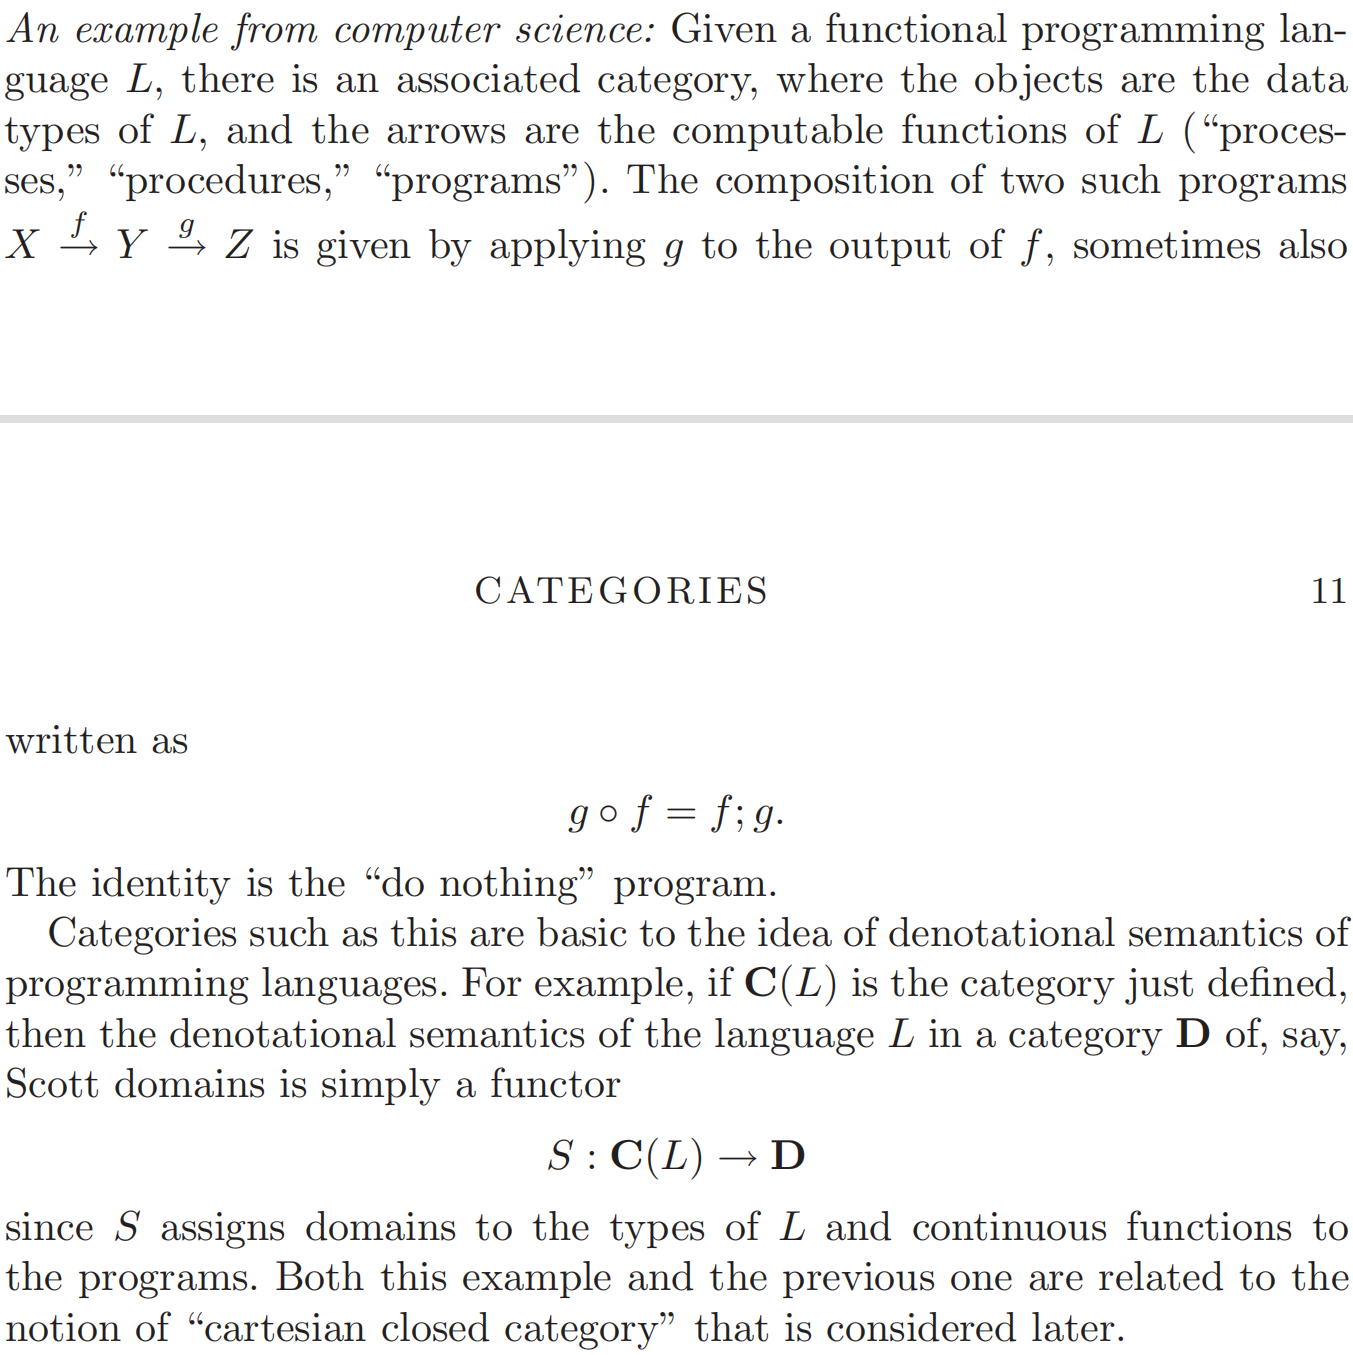
\includegraphics[width=0.7\linewidth]{1.4_11}
		\caption{}
		\label{fig:1}
	\end{figure}
	
	\subsection{Isomorphisms}
	\paragraph{Definition 1.3}
	while there are ``bijective homomorphisms''
	between non-isomorphic posets.
	
	\blue{The inverse must also be homomorphism?}
	
	\paragraph{Theorem 1.6}
	

	\[\red{f,h\in \bar{C}}, \blue{g\circ f,g\circ h\in \bar{D}}.\]
	\begin{centikzcd}[
			remember picture,
			every matrix/.append style={name=arrows}
		]
		X\ar[d,red,"f"']\ar[rd,blue,"g\circ f"]&\\
		C\ar[r,red!50!blue!100,"g"]&D&&\red{\bar{C}}\ar[r,red!50!blue!100,"\bar{g}"] & \blue{\bar{D}} \\
		Y\ar[u,red,"h"]\ar[ru,blue,"g\circ h"']&
	\end{centikzcd}
	%\begin{tikzpicture}[remember picture, overlay]
	%	\def\mid{40}
	%	\draw[red,rounded corners] ([xshift=0pt]arrows.south west) rectangle ([xshift=17.5pt, yshift=15pt]arrows.north west)
	%	node [below left] {$\bar{C}$};
	%\end{tikzpicture}

	If every category (large or small) was isomorphic to a concrete (small) category,
	what make those large?
	
	\blue{The assumption is wrong. Only small categories are isomorphic to a small category.}
	See this: \ref{sec:too_many_arrows}.
	
	\blue{Also see Warning 1.13 that small does not imply concrete and neither is the converse.} 
		
	\paragraph{Remark 1.7}
	\subparagraph{Test object}
	
	\red{What does this mean}
	\begin{figure}[H]
		\centering
		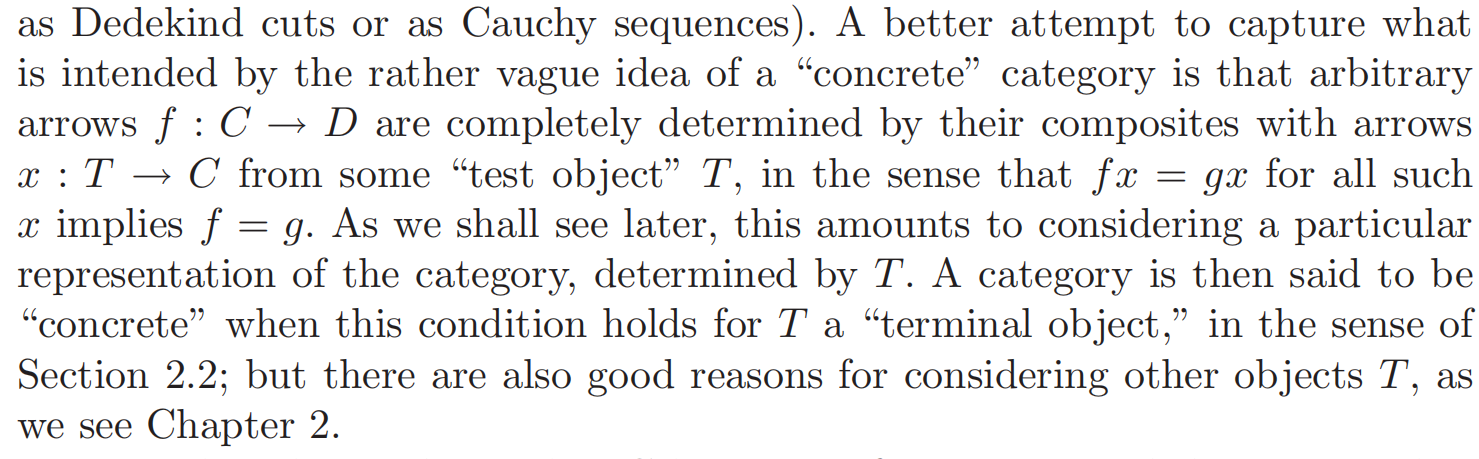
\includegraphics[width=0.7\linewidth]{1.5_1.7}
		\caption{}
		\label{fig:2}
	\end{figure}
	
	\subparagraph{Too many arrows}\label{sec:too_many_arrows}
	\blue{If the arrows in the category is too large to form a set, then it might not be isomorphic to a small category?}
	
	\subsection{Constructions on categories}
	\paragraph{3 The arrow category}
	
	\begin{centikzcd}
		A\ar[r,"g_1"]\ar[d,"f"]&A'\ar[r,"h_1"]\ar[d,"f'"]&A''\ar[d,"f''"]\\
		B\ar[r,"g_2"]&B'\ar[r,"h_2"]&B''
	\end{centikzcd}
	\paragraph{4 Slice category}
	
	\subparagraph{Definition of $\bfC/(-)$}
	
	\[ \bfC/(-)\colon\bfC\to\mathbf{Cat}\colon C\to\bfC/C\colon g\to g_*. \]
	
	\subparagraph{Cat to Sets}
	
	\blue{the forgetful functor $U \colon \mathbf{Cat} \to \mathbf{Sets}$
	that takes a category to its underlying set of objects.}

	Do the objects form a set? Guaranteed?
	\href{https://math.stackexchange.com/questions/750731/is-there-a-category-of-categories}{Is there a category of categories?}
	
	\blue{Yes, because $\mathbf{Cat}$ is defined as the category of \textit{small} categories.
		There is no category of all categories. Likewise, there is no ``set of all sets'' or ``class of all classes''}
	
	\red{But is $\bfC/C$ a small category? If and only if $\bfC$ is small?}
	
	\subparagraph{Principal ideal}
	
	the slice category P/p is just the \red{``principal ideal'' (what does this mean? what is down arrow?)} $\downarrow (p)$ of elements $q \in P$
	with $q \le p$.
	
	\paragraph{Example 1.8}
	
	$1=\set{*}$ is mapped to the distinguished point of sets in $\mathbf{Sets}_*$.
	
	\subsection{Free categories}
	\paragraph{Free monoid}
	The Kleene closure of $A$ can be thought as
	\[ \set{\text{Empty word}} \sqcup A \sqcup A\times A \sqcup \dots ,  \]
	where $\times $ is the Cartesian product.
	
	A free monoid can be thought as some monoid isomorphic to the  Kleene closure of some set.
	
	A free monoid can be defined as a monoid whose non-identity elements can be uniquely written as a product of its generating elements?
	
	\paragraph{UMP}
	
	The mapping $i\colon A\to |M(A)|$ must be injection because otherwise there is no monoid
	homomorphism from $M(A)$ to $A^*$, the Kleene closure.
	
	\paragraph{Free category}
	
	\red{Does edges and vertices always form a set?}
	
	\subsection{Foundations: large, small, and locally small}
	
	\paragraph{Definition 1.12}
	
	\subparagraph{The category of sets is locally small}
	\label{par:sets_locally_small}
	
	Given two \textit{sets} $X$ and $Y$,
	an ordered pair $(x,y)\in X\times Y$ can be viewed as an element in $\power\power(X\cup Y)$
	(by Kuratowski's definition).
	Therefore, a function $f\colon X\to Y$ as a subset of $X\times Y$ is an element of $\power\power\power(X\cup Y)$.
	In conclusion, the set of all functions from $X$ to $Y$ is a subset of $\power\power\power(X\cup Y)$,
	and therefore based on the axiom of replacement and power set, it is a (small) set.
	
	\subparagraph{The category of small categories is locally small}
	
	Since the objects and arrows form two sets, so does their disjoint union.
	
	Therefore, a functor can be viewed as a function between two sets, and therefore $\mathbf{Cat}$ is locally small.
	
	\subparagraph{Non-locally small category}
	
	\href{https://mathoverflow.net/questions/3278/whats-a-reasonable-category-that-is-not-locally-small}{Examples}
	
	\subsection{Exercises}
	\paragraph{2}
	\subparagraph{a}
	
	Yes, $\mathbf{Rel}\cong\opp{\mathbf{Rel}}$.
	\subparagraph{b}
	$\mathbf{Sets}$ is not isomorphic to its opposite because
	all terminal objects must be mapped to an initial object as
	a terminal object in the opposite,
	than mapped back to a terminal object.
	
	But there are infinite terminal objects in $\mathbf{Sets}$
	(singletons) and only one initial object (the empty set).
	
	\subparagraph{c}
	
	\blue{For the whole power set it should be true?}
	
	Any subset is mapped to its complement.
	
	This is not necessarily true for a subset of the power set.
	
	\paragraph{3}
	\subparagraph{c}
	There is a bijective monotone function (functor) from a discrete (small) category
	(which is a poset)
	 to a non-discrete poset category of same objects.
	
	But this is not isomorphism.
	
	\paragraph{5}
	
	\[F\colon\bfC/C\to\bfC^{\rightarrow}\]
	is the trivial functor which maps arrows to itself.
	
	\paragraph{6}
	
	\[C/\bfC \cong \opp{(\opp{\bfC}/C)}. \]
	The only difference is the objects are arrows with opposite directions.
	
	\begin{centikzcd}
		X\ar[rr,"a"]\ar[rd,"f"']&&X'\ar[ld,"f'"] \\
		&C\ar[rd,"g'"]\ar[ld,"g"']&\\
		Y\ar[rr,"b"']&&Y'\\
	\end{centikzcd}

	\paragraph{7}
	
	%\subparagraph{}
	For any positive integer $n$,
	\[ F\colon\mathbf{Sets}/n\to \mathbf{Sets}^n, \]
	\[ (f\colon X\to \set{a_1,\dots,a_n} )\mapsto (f^{-1}(a_1),\dots,f^{-1}(a_n)).  \]
	\[  (f\to g)\mapsto (f^{-1}(a_1)\to g^{-1}(a_1),\dots, f^{-1}(a_n)\to g^{-1}(a_n)  ) .\]
	
	\begin{enumerate}
		\item 
		First, the image is contained in the codomain.
		
		\item
		It is a functor.
		
		\item \red{It is isomorphism?}
	\end{enumerate}

	\paragraph{8}\label{par:preorder_category}
	
	In the preorder category $P(\bfC)$,
	any information encoded in the arrows is forgotten,
	only the domain and codomain is kept.
	
	\begin{centikzcd}
		 A \ar[r,bend left=45,"f_1"]\ar [r,"f_2"] \ar[loop left,"1_A"] \ar[loop,in=140,out=220,looseness=10,"i_A"]
		 &B\ar[l,shift left=2,"g"] &C\ar[l,"h"']\\
		 A \ar[r,shift left=1,"f'"] \ar[loop left,"1_A"] 
		 &B\ar[l,shift left=1,"g'"] &C\ar[l,"h'"']\\
	\end{centikzcd}

	$P(1_A)=P(i_A)=1_A, P(f_1)=P(f_2)=f'$.
	
	Since any functor preserves domain and codomain,
	any functor can be mapped as an arrow between two preorder sets.
	
	For example, given two categories $\bfC,\bfD$,
	if the functor $F$ maps \textit{any} arrow in $\bfC$ $(X\to Y)$ to \textit{an} arrow in $\bfD$ $(F(X)\to F(Y))$,
	then the it maps \textit{the} arrow in $P(\bfC)$ $(X\to Y)$ to \textit{the} arrow in $P(\bfD)$ $(F(X)\to F(Y))$.
	
	The identity is preserved since $A\le A$, the composite is preserved due to the transitivity $A\le B\land B\le C\implies A\le C$.
	
	Let $I$ be the inclusion, then $P\circ I=1$ but $I\circ P\ne 1$.
	
	\paragraph{9}
	\subparagraph{c}
	
	\begin{eqlong}
		a\to a&: 1_a,\\
		a\to b&: e,\\
		b\to b&: 1_b,\\
		b\to c&:f,\\
		c\to c&:1_c,\\
		a\to c&:f\circ e,g,\\
	\end{eqlong}

	\subparagraph{d}
	The only arrow related to $d$ is $1_d$.
	
	\[a\to a:1_a,(he)^n, (gfe)^n,\]
	\[b\to b:1_b,(eh)^n, (egf)^n,\]
	\[c\to c:1_c,(feg)^n.\]
	\[a\to b:e\circ (a\to a); b\to a: (h \lor gf)\circ (b\to b).\]
	
	\paragraph{10}
	
	\red{Can you have a directed graph with only 1 vertex, but 6 edges on the same vertex?
	or only 2 vertices and 3 edges for each direction connecting these?}

	\paragraph{11}
	\subparagraph{b}
	Assume $\forall A\in \mathbf{Sets}\, \exists! i_A\colon A \to |M(A)|$ as a UMP
	(existence: \ref{prop:Kleene_is_free}, uniqueness: just pick any one for each $A$ and fix it),
	then \[ \forall (f\colon A\to B)\, \exists! i_B\circ f\, \exists! M(f) \]
	(existential uniqueness of $i_B\circ f$ is given by \ref{prop:exist_unique}) such that the following diagram commutes.
	\begin{centikzcd}
		\mathbf{Mon}& M(A)\ar[r,red,dashed,"\exists!M(f)"]&M(B)\\
		\mathbf{Sets}& \vert M(A) \vert \ar[r,red,"|M(f)|"]& \vert M(B)\vert \\
		&A\ar[r,"f"]\ar[ru,red,"i_B\circ f"]\ar[u,red,"i_A"]& B\ar[u,"i_B"]
	\end{centikzcd}

	Let $f=1_A$, and $B=A$.
	Since $1_{|M(A)|}\circ i_A = i_A\circ 1_A$ and $|1_{M(A)}|=1_{|M(A)|}$,
	therefore $M(1_A)=1_{M(A)}$.
	
	Associativity:
	\begin{centikzcd}
		\mathbf{Mon}& M(A)\ar[r,red,dashed,"\exists!M(f)"]&M(B)\ar[r,dashed,blue,"\exists! M(g)"]&M(C)\\
		\mathbf{Sets}& \vert M(A) \vert \ar[r,red,"|M(f)|"]& \vert M(B)\vert \ar[r,blue,"|M(g)|"]& \vert M(C)\vert \\
		&A\ar[r,"f"']\ar[ru,red,"i_B\circ f"']\ar[u,red,"i_A"]& B\ar[u,blue,"i_B"]\ar[ru,blue,"i_C\circ g"']\ar[r,"g"']&C\ar[u,"i_C"]
	\end{centikzcd}

	\paragraph{14}
	\red{TODO}
	
	\section{Abstract structures}
	
	\subsection{Epis and monos}
	\paragraph{Example 2.3}
	\subparagraph{Prove $h$ monic implies $|h|$ monic}
	
	\[ h\bar{x}\ne h\bar{y}\implies|h|x\ne|h|y, \]
	due to UMP of $M(1)$.
	(If $|h|x=|h|y$, then there exists non-unique maps $h\bar{x}, h\bar{y}$ corresponding it,
	which contradicts UMP.)
	
	
	\subparagraph{Converse}
	
	If $f,g : X \to M$ are any distinct
	homomorphisms, then $|f|, |g| : |X|\to|M|$ are distinct functions.
	The converse is true, only if there is a monoid homomorphism corresponding to the underlying function.
	This is to say, function to monoid homomorphism mapping is injective but not surjective.
	
	\paragraph{Example 2.4}
	
	Because there is at most 1 arrow between 2 objects!
	\subsubsection{Sections and retractions}
	\paragraph{Definition 2.7}
		
	$A$ is ``smaller'' than $X$.
	
	\blue{Functors preserve split epis and split
	monos, but do not preserve all the epis.}

	\paragraph{Projective}
	\red{What does projective mean?}
	
	\subparagraph{Epi into projective object splits}
	
	Let $P$ be the projective object and $e\colon E \twoheadrightarrow P$ the epi.
	Since $1_P$ must exist, therefore
	by definition of projective object, $\exists m$ such that
	\begin{centikzcd}
		&E\ar[d,two heads,"e"]\\
		P\ar[ru,dashed,tail,"\exists m"] \ar[r,"1_P" ] & P\\
	\end{centikzcd}
	Therefore $e$ splits and $m$ is mono
	(by definition of split epi).
	
	\subparagraph{More free}
	Projective objects may be thought of as having a more ``free'' structure, thus
	permitting ``more arrows''.
	
	I guess this means: for any epi and any arrow from a projective object sharing the codomain,
	there must be another arrow from the projective object to the domain of the epi,
	so there will be ``more'' arrows than ``necessary''.
	
	\subparagraph{AC vs projective}
	\label{par:split_epi_projective}
	
	\begin{prop}
		\blue{If all epis are split, then all objects are projective.}
	\end{prop}

	\begin{proof}
		Because for any epi $e\colon E\twoheadrightarrow X$
		there is a mono $m\colon X\rightarrowtail E$ such that $em=1_X$, therefore for any $f\colon P \to X$,
		there must be $\bar{f}=m\circ f$ such that the following diagram commutes.
		\begin{centikzcd}
			&E\ar[rd,two heads,"e"]&\\
			P\ar[r,"f"]\ar[ru,dashed,"m\circ f"]&X\ar[r,"1_X"]\ar[u,tail,"m"]&X
		\end{centikzcd}
	\end{proof}

	\red{It follows that
		free objects in many (but not all!) categories of algebras then are also projective.}

	\subparagraph{Retract of projective object}
	\label{par:retract_projective}
	\begin{prop}
		Any retract of a projective object is also
		projective.
	\end{prop}
	\begin{proof}
		Let $R$ be a retract of a projective object $P$,
		and let $rs=1_R$.
		Then given any epi $e\colon E\twoheadrightarrow X$, 
		and any $f\colon R\to X$, the following diagram must commute.
		\begin{centikzcd}
			&&E\ar[d,red,two heads,"\forall e"]\\
			&P\ar[r,red,"f\circ r"]\ar[ru,dashed,red,"\exists \overline{f\circ r}"]\ar[d,two heads,"r"]&X\\
			R\ar[ru,tail,"s"]\ar[r,"1_R"]&R\ar[ru,red!50!blue!100,"\forall f"'] &
		\end{centikzcd}
		
		And therefore $f$ lifts across $e$ to $\overline{f\circ r} \circ s$.
	\end{proof}
	
	\subsection{Initial and terminal objects}
	
	\paragraph{Example 2.11}
	\subparagraph{3 Rings}
	In $\mathbf{Rings}$ (commutative with unit), the ring $\inte$ of integers is initial.
	
	For any finite rings, they might not be homomorphic to other finite rings of different size (\eg, $\field_q$).
	
	$\inte$ is the smallest infinite ring. Since $0$ must be mapped to $0$ and so is $1$, there exists a unique ring homomorphism
	from $\inte$.
	\subsection{Generalized elements}
	
	\paragraph{Ultrafilter}
	a filter $F$ is an ultrafilter just if for every element $b \in B$, either $b \in F$ or $\neg b \in F$,
	and not both (exercise!).
	
	\paragraph{Prime ideal}
	Ring homomorphisms $A \to Z$ into the initial ring $Z$ play an analogous and
	equally important role in algebraic geometry. They correspond to so-called prime
	ideals, which are the ring-theoretic generalizations of ultrafilters.
	\paragraph{Example 2.12}
	\subparagraph{3}
	\[f=g\iff f1_C=g1_C.\]
	\paragraph{Example 2.13}
	\red{$\Hom(X, -)$ is always a functor, and functors always preserve isos.}
	\paragraph{Example 2.14}
	\subparagraph{Natural number is the revealing object}
	
	
	\begin{centikzcd}
		\mathbf{Mon}& M(1)\ar[r,dashed,"\exists \bar{x}"]&M\\
		\mathbf{Sets}& \vert M(1) \vert \ar[r,"|\bar{x}|"]& \vert M\vert \\
		&\set{*} \ar[ru,"\forall x"']\ar[u,"i"]&
	\end{centikzcd}

	For any $x\in |M|$, there is a function $x\colon *\mapsto x$.
	To make the diagram commute, $|\bar{x}|\big( i(*)\big)= x$.
	
	This uniquely corresponds to a monoid homomorphism $\bar{x}\colon i(*)\mapsto x$.
	Therefore, every element in $|M|$ can be reached by a monoid homomorphism from $M(1)$.
	And $\nat$ is isomorphic to $M(1)$.
	\subparagraph{Bijection}
	From above, we clearly see that different $x$ correspond to different monoid homomorphism $\bar{x}\colon i(*)\mapsto x$,
	and exactly one for each.
	Therefore \[\card{\Hom_{\mathbf{Sets}}(1,|M|)}\le \card{\Hom_{\mathbf{Mon}}(M(1),|M|)}.\]
	
	On the other hand, for any monoid homomorphism $f\colon M(1)\to M$,
	there is uniquely $x=|f|\circ i$ which makes the diagram commute.
	Different $f$ must correspond to different $x$, otherwise it contradicts the UMP axiom.
	
	\paragraph{Universal Property}
	\subparagraph{Bijection in general}
	
	\begin{prop}\label{prop:exist_unique}
		Given a commutative diagram in category $\bfC$
		\begin{centikzcd}
			A\ar[r,"f"]& B\ar[d,"g"]\\
			&C
		\end{centikzcd}
		there \textit{exists} a \textit{unique} commutative diagram in $\bfC$
		\begin{centikzcd}
			A\ar[r,"f"]\ar[rd,dashed,"\exists! h"'] & B\ar[d,"g"]\\
			&C
		\end{centikzcd}
		where $h$ is uniquely determined as $g\circ f$.
	\end{prop}
	\begin{proof}
		Given the definition of commutative diagram,
		if $h$ exist, it must be $g\circ f$ (uniqueness).
		
		Given the axiom of category, $g\circ f$ must exist if both $f$ and $g$ exist (existence).
	\end{proof}
	\begin{rem*}
		Therefore, such edge can be arbitrarily added or deleted without loss of generality.
	\end{rem*}
	\begin{rem*}
		%Note that $g$ might not be uniquely determined by $f$ and $h$ unless $f$ is epi.
		Note that $g$ is uniquely determined by $f$ and $h$ if and only if $f$ is epi.
		\begin{centikzcd}
			A\ar[r,two heads,"f"]\ar[rd,"h"'] & B\ar[d,dashed,"\exists g \implies \exists! g"]&&
			A\ar[r,dashed,"\exists f \implies \exists ! f"]\ar[rd,"h"'] & B\ar[d,tail,"g"]\\
			&C&&&C
		\end{centikzcd}
	\end{rem*}
	
	\begin{def*}[universal property]
		Let $F\colon \bfC\to \bfD$ be a functor between categories $\bfC$ and $\bfD$,
		and let $X\in\ob(\bfD), A,A'\in\ob(\bfC)$.
		
		A \textbf{universal morphism from $X$ to $F$} is a unique pair $(A,u\colon X\to F(A))$ in $D$
		such that any morphism of the form $f\colon X\to F(A')$ in $D$, there \textit{exists a unique} morphism
		$h\colon A\to A'$ in $C$ such that $f=F(h)\circ u$, \ie, the following diagram commutes:
		\begin{centikzcd}
			\bfC & \blue{A} \ar[dashed,r,"\exists ! h"] & A'\\
			\bfD & F(\blue{A}) \ar[dashed,r,"\exists F(h)"] & F(A')\\
			& X \ar[u,red,"u"] \ar[ur,"\forall f"'] &
		\end{centikzcd}
	
		A \textbf{universal morphism from $F$ to $X$} is a unique pair $(A,u\colon  F(A)\to X)$ in $D$
		such that any morphism of the form $f\colon  F(A')\to X$ in $D$, there \textit{exists a unique} morphism
		$h\colon A'\to A$ in $C$ such that $f= u\circ F(h)$, \ie, the following diagram commutes:
		\begin{centikzcd}
			\bfC & \blue{A} \ar[dashed,from=r,"\exists ! h"'] & A'\\
			\bfD & F(\blue{A}) \ar[dashed,from=r,"\exists F(h)"'] & F(A')\\
			& X \ar[from=u,red,"u"'] \ar[from=ur,"\forall f"] &
		\end{centikzcd}
	\end{def*}

	\begin{prop}\label{prop:same_arrows}
		Given two locally small categories $\bfC$ and $\bfD$,
		if $(A,u\colon X\to F(A))$ is a universal morphism from $X$ to $F$,
		then $\forall A'\in \ob(\bfC)$ there is a bijection for hom-sets
		\[ \Hom_\bfC(A,A')\cong \Hom_\bfD(X,F(A')). \]
	\end{prop}
	\begin{proof}
		From the definition of universal morphism,
		there is a unique $h\in \Hom_\bfC(A,A')$ corresponding
		each $f\in \Hom_\bfD(X,F(A'))$, and let the mapping be
		\[ G\colon\Hom_\bfD(X,F(A'))\to  \Hom_\bfC(A,A')\colon f\to h  \]
		such that the definition diagram commutes.
		
		Conversely, for any $g\in \Hom_\bfC(A,A')$, there exists a unique
		morphism $ F(g) \circ u $ (\ref{prop:exist_unique}) such that the definition diagram commutes,
		therefore
		\[ G'\colon\Hom_\bfC(A,A')\to  \Hom_\bfD(X,F(A')) \colon g\to F(g) \circ u   \]
		is another mapping.
		
		Since the diagram commutes, they must be inverse, \ie,
		\[ GG'=1, G'G=1. \]
	\end{proof}
	\begin{rem*}
		Different $h$ corresponds to different $f$
		because otherwise it contradicts the universal property.
		
		Different $f$ corresponds to different $h$
		because the composite $F(g)\circ u$ is uniquely determined by its components $F(g)$ and $u$.
		And there is no other morphism $X\to F(A')$ that makes the diagram commute (\ref{prop:exist_unique}).
	\end{rem*}

	\begin{cor}\label{prop:same_arrows_from_F_to_X}
		Given two locally small categories $\bfC$ and $\bfD$,
		if $(A,u\colon F(A)\to X)$ is a universal morphism from $F$ to $X$,
		then $\forall A'\in \ob(\bfC)$ there is a bijection for hom-sets
		\[ \Hom_\bfC(A',A)\cong \Hom_\bfD(F(A'),X). \]
	\end{cor}

	\subparagraph{Properties of universal morphism}
	\label{par:universal_morph_prop}
	
	See definition here: \ref{universal property}.
	
	\begin{prop}\label{prop:UMP_mono_epic}
		Given categories $\bfC,\bfD$, a functor $F\colon \bfC\to \bfD$, and a universal morphism from $X$ to $F$
		\[ \big(A,u\colon X\to F(A)\big) ;\]
		if \[ \exists f\colon X\rightarrowtail F(B) ,\]
		then $u$ is monic.
		
		The dual property claims that
		given a universal morphism from $F$ to $X$
		\[ \big(A,u\colon F(A)\to X\big) ;\]
		if \[ \exists f\colon X\twoheadrightarrow F(B) ,\]
		then $u$ is epic.
	\end{prop}
	\begin{proof}
		See \ref{par:trig_mono}.
		
		If the following diagram commutes, then $i=j$.
		\begin{centikzcd}
			&F(A)\ar[r,dashed,"\exists! F(h)"]&F(B)\\
			Y\ar[r,shift left,"i"]\ar[r,shift right, "j"']&X\ar[u,tail,"u"]\ar[ur,tail,"f"']&
		\end{centikzcd}
	\end{proof}
	\begin{rem*}
		There exist non-monic universal morphism from $X$ to $F$.
		Let $A=\set{0}$ be the only object in $\bfC$,
		$\bfD$ be a subcategory of $\mathbf{Sets}$ with $A$ and $X=\set{-1,1}$ as objects and functions as arrows.
		Define the functor $F\colon\bfC\to\bfD$ as $F(A)=A\in \bfD$. Then a universal morphism from $X$ to $F$
		$(A,u\colon X\to A)$ is not monic:
		\begin{centikzcd}
			\ar[loop left,"1_X"]\ar[loop,in=150,out=210,looseness=10,"-1_X"]X \ar[r,"\exists ! u"] & A=F(A)\ar[loop right,"\exists! 1_A=F(1_A)"]
		\end{centikzcd}
	\end{rem*}
	
	\begin{cor}
		Given categories $\bfC,\bfD$, a functor $F\colon \bfC\to \bfD$. Let
		\[ \big(A,u\colon F(B)\to F(A)\big) \]
		be a universal morphism from $F(B)$ to $F$, then $u$ is monic.
		
		Let
		\[ \big(A,u\colon F(A)\to F(B)\big) \]
		be a universal morphism from $F$ to $F(B)$, then $u$ is epic.
	\end{cor}
	\begin{proof}
		$\exists 1_{F(B)}\colon F(B)\to F(B)$ that is both epic and monic.
		And \ref{prop:UMP_mono_epic}.
	\end{proof}
	
	\begin{cor}\label{cor:inj_UMP_set_to_U}
		Let $U\colon \mathbf{Mon}\to \mathbf{Sets}$ be the forgetful functor,
		then for any universal morphism from a set $X$ to $U$
		\[ \big(A, i\colon X \to U(A) \big), \]
		$i$ is monic (injective).
	\end{cor}
	\begin{proof}
		For any set $X$, its power set $\power(X)$ is also a set (axiom of power set),
		as well as a monoid under intersection (or union or symmetric difference).
		
		There is an injection $f\colon X\rightarrowtail\power(X)\colon x\mapsto \set{x}$.\\
		$i$ is monic followed by \ref{prop:UMP_mono_epic}.
	\end{proof}

	\begin{prop}\label{prop:UMP_morph2morph}
		Given categories $\bfC,\bfD$, a functor $F\colon \bfC\to \bfD$, and a universal morphism from $X$ to $F$
		\[ \big(A,u\colon X\to F(A)\big) \]
		or
		a universal morphism from $F$ to $X$
		\[ \big(A,u\colon F(A)\to X\big) ;\]
		then \[ \forall f\colon A\to A [F(f)=1_{F(A)}\iff f=1_A].\]
	\end{prop}
	\begin{proof}
		$\Longleftarrow$: required by the definition of functor.
		
		$\Longrightarrow$: (wlog, consider universal morphism from $X$ to $F$)
		\begin{centikzcd}
			\bfC& A\ar[r,dashed,"\exists! f"] & A\\
			\bfD& F(A) \ar[r,"F(f)"]& F(A)\\
			& X\ar[u,"u"]\ar[ur,"u"']&
		\end{centikzcd}
		Since $f=1_A$ makes the above diagram commute, based on UMP,
		\[\forall g \colon A\to A [F(g)=F(f)=1_{F(A)} \implies g=f=1_A].\]
	\end{proof}
	\begin{rem*}
		However, it is possible that \[ \exists f\colon A\to A [ f\ne 1_A].\]
	\end{rem*}

	\begin{prop}
		Given categories $\bfC,\bfD$, a functor $F\colon \bfC\to \bfD$, and a universal morphism from $X$ to $F$
		\[ \big(A,u_A\colon X\to F(A)\big) ;\]
		then $\exists u_B$ such that \[ \big(B,u_B\colon X\to F(B)\big) \]
		is a universal morphism from $X$ to $F$ iff
		%$A\iso B$ 
		$A\cong B$
		in $\bfC$.
		
		The dual property claims that
		given a universal morphism from $F$ to $X$
		\[ \big(A,u_A\colon F(A)\to X\big) ;\]
		then $\exists u_B$ such that
		\[ \big(B,u_B\colon  F(B)\to X\big) \]
		is a universal morphism from $F$ to $X$ iff
		%$A\iso B$ 
		$A\cong B$
		in $\bfC$.
	\end{prop}
	\begin{proof}
		Necessity:
		UMP determines objects up to isomorphism.
		\begin{centikzcd}
			\bfC& &A\ar[rr,shift left,dashed,red,"\exists!f"] \ar[loop left,red!75!blue!100,"\exists! g\circ f"]&&
			 B\ar[ll,shift left,dashed,blue,"\exists!g"]\ar[loop right,blue!75!red!100,"\exists! f\circ g"]\\
			%%%%%%%%%%
			\bfD && F(A)\ar[loop left,red!75!blue!100,"1_{F(A)}"]\ar[rr,shift left,red,"\exists F(f)"]
			&& F(B)\ar[ll,shift left,blue,"\exists F(g)"]\ar[loop right,blue!75!red!100,"1_{F(B)}"] \\
			%%%%%%%%%%
			&&&X\ar[ul,red!75!blue!100,"u_A"]\ar[ur,blue!75!red!100,"u_B"']&
		\end{centikzcd}
		Per UMP of $u_A$, $\exists! f$ such that the \red{red} diagram commutes:
		\[ F(f)\circ u_A=u_B. \]
		Per UMP of $u_B$, $\exists! g$ such that the \blue{blue} diagram commutes:
		\[ F(g)\circ u_B=u_A. \]
		Therefore we have (by plugging in the above equations and applying the axiom of functor):
		\begin{eqlong}
			1_{F(A)}\circ u_A &= u_A  = F(g)\circ \big(F(f)\circ u_A\big) = F(g\circ f)\circ u_A,\\
			1_{F(B)}\circ u_B &= u_B  = F(f)\circ \big(F(g)\circ u_B\big) = F(f\circ g)\circ u_B,\\
		\end{eqlong}
		%Since the total diagram commute, we have \[F(g)\circ F(f)=1_{F(A)},F(f)\circ F(g)=1_{F(B)}.\]
		Per UMP of $u_A$ and $u_B$ (\ref{prop:UMP_morph2morph}), we have
		\[g\circ f = 1_A, f\circ g=1_B.\]
	
		Sufficiency:
		Given any isomorphism $f\colon A\iso B$ in $\bfC$ (iso is also epic), the following diagram commutes
		for any object $C$ in $\bfC$ and any arrow $c\colon X\to F(C)$ in $\bfD$.
		\begin{centikzcd}
			\bfC& A \ar[two heads,r,"f"']\ar[rr,red,bend left,"\exists! h"] & B \ar[r,dashed,"\exists! g"'] & C\\
			\\
			\bfD& F(A)\ar[rr,bend left,red,"F(h)"]\ar[r,"F(f)"]&F(B)\ar[r,dashed,"\exists F(g)"]&F(C)\\
			&& X\ar[lu,red,"u_A"]\ar[u,"\exists u_B"']\ar[ur,red,"\forall c"']&
		\end{centikzcd}
		where $u_B=F(f)\circ u_A$.
		
		Per UMP of $u_A$, the red diagram commutes. Since $f$ is epic, $g$ is uniquely determined by $f$ and $h$.
		Since $f$ is isomorphism, $g$ exists as $h\circ f^{-1}$.
		Therefore $\exists! g$ such that the diagram commutes, \ie, $(B,u_B)$ is universal morphism.
	\end{proof}
	\begin{rem*}
		There might be different isomorphism between $A$ and $B$, but only one such that the diagram commutes with $u_A$ and $u_B$. 
		
		Generally $F(f\circ g)=1_{F(B)}$ does not imply $f\circ g=1_B$.
		Consider a small category $\bfC$ containing two objects:
		\[ A=\set{0,1},B=\set{0,1,2}, \]
		and arrows
		\[ \begin{aligned}
			i_A &\colon A\to B\colon i\mapsto i,\\
			f_1 &\colon B\to A\colon i\mapsto i\bmod 2,\\
			f_2 &\colon B\to A\colon i\mapsto \min(1,i),\\
		\end{aligned} \]
		and identity arrows and composites.
		Construct a (preorder) category $\bfD$ with functor $F\colon \bfC\to\bfD$ as
		\begin{centikzcd}
			F(A)\ar[rr,shift left,"F(i_A)"]&&\ar[ll,shift left,"F(f_1)=F(f_2)"]F(B)\\
			&\ar[ul,"u_A"]X\ar[ur]&
		\end{centikzcd}
		Even though $(A,u_A)$ is a UMP, we still have $F(f_1)F(i_A)=1_{F(B)}$, $f_1i_A\ne 1_B$.
	\end{rem*}
	
	
	\subparagraph{Initial and terminal objects are defined by universal property}
	
	Given a category $\bfC$, define a category $\bfD$ whose objects are equivalent to objects in $\bfC$.
	Define $\bfD$ such that
	there is \textit{exactly one} arrow between any two objects in $\bfD$ (easy to prove $\bfD$ is a valid category,
	see \ref{par:preorder_category}).
	Define a functor $F\colon \bfC\to\bfD$ such that for any arrow $f\colon A\to B$ in $\bfC$,
	the corresponding arrow is \textit{the} arrow $F(f)\colon F(A)\to F(B)$ in $\bfD$ (easy to prove $F$ is a functor if $\bfD$ is a valid category).
	
	Then an initial object $I$ of $\bfC$ is defined by
	a universal morphism from $F(I)$ to $F$: $(I,1_{F(I)}\colon F(I)\to F(I))$.
	\begin{centikzcd}
		\bfC&&\blue{I}\ar[r,dashed,"\exists ! h"]&A'\\
		\bfD&&F(\blue{I})\ar[loop left,red,"1_{F(I)}"]\ar[r,shift left,dashed,"\exists ! F(h)"]\ar[r,shift right,"\forall f"']& F(A')\\
		%F(I)
	\end{centikzcd}
	In the definition (\ref{universal property}), $X = F(I), A = I, u = 1_{F(I)}$.
	
	Because for any object $A'$ in $\bfC$, there is \textit{exactly one} arrow $f\colon X=F(I)\to F(A')$ in $\bfD$,
	so there exists \textit{exactly one} arrow from $A=I$ to any object $A'$ in $\bfC$ (\ref{prop:same_arrows}).
	
	%Given a category $\bfC$, an initial object $I$ of $\bfC$ is defined by the 
	%a universal morphism from $I$ to $1_\bfC$: $(I,1_I\colon I\to 1_\bfC(I))$
	%where $1_\bfC$ is the identity functor.
	%\begin{centikzcd}
	%	I\ar[loop left,"1_I"]\ar[r,dashed,"\exists ! h"]& A'
	%\end{centikzcd}
	%In the definition (\ref{universal property}), $\bfD = \bfC, X = I, F = 1_\bfC, A = I, u = 1_I$.
	
	A terminal object $T$ of $\bfC$ is defined by a
	universal morphism from $F$ to $F(T)$: $(T,1_{F(T)}\colon F(T)\to F(T))$
	\begin{centikzcd}
		\bfC&&\blue{T}\ar[from=r,dashed,"\exists ! h"']&A'\\
		\bfD&&F(\blue{T})\ar[loop left,red,"1_{F(T)}"]\ar[from=r,shift right,dashed,"\exists ! F(h)"']
		\ar[from=r,shift left,"\forall f"]& F(A')\\
		%F(I)
	\end{centikzcd}
	In the definition (\ref{universal property}), $X = F(T), A = T, u = 1_{F(T)}$.
		
	Because for any object $A'$ in $\bfC$, there is \textit{exactly one} arrow $f\colon  F(A')\to X=F(T)$ in $\bfD$,
	so there exists \textit{exactly one} arrow from any object $A'$  to $A=T$ in $\bfC$ (\ref{prop:same_arrows_from_F_to_X}).
	
	\subsection{Products}
	\paragraph{Arrows out of the product}
	\red{To be sure, they are related to the notion of an
	``exponential'' $Y^B$, via ``currying'' $\lambda f : A \to Y^B$; we discuss this further in
	Chapter 6.}
	\paragraph{Product is defined by universal property}
	
	\subparagraph{Cumbersome definition}
	Given a category $\bfC$, and a product diagram in $\bfC$
	\begin{centikzcd}
		A&P\ar[l,"p_1"']\ar[r,"p_2"]&B
	\end{centikzcd}
	define a copy $\bfD$ of $\bfC$, with one additional object, denoted $(A, B)$.
	The only arrow from $(A,B)$ to itself is the identity arrow $1_{(A,B)}$.
	There is no arrow from $(A,B)$ to other different objects in $\bfD$.
	For any object $C$ in $\bfC$, and any arrows $f\colon C\to A, g\colon C\to B$ in $\bfC$,
	define an arrow $(f,g)\colon C\to (A,B)$ in $\bfD$.
	If, for example, there are $3$ arrows $C\to A$, and $2$ for $C\to B$ in $\bfC$,
	then there will be $6$ for $C\to (A,B)$ in $\bfD$.
	
	We now define the composite to make $\bfD$ a category.
	For any $h\colon D\to C$ in $\bfC$ and any $(f,g)\colon C\to (A,B)$ in $\bfD$,
	$(f,g)\circ h\define (f\circ h,g\circ h)$ is an arrow from $D$ to $(A,B)$
	because both $f\circ h\colon D\to A$ and $g\circ h\colon D\to B$ exist in $\bfC$.
	\begin{centikzcd}
		D \ar[r,"h"] \ar[rd,dashed,"{(f\circ h, g\circ h)}"'] & C \ar[d,"{(f,g)}"] \\
		& (A,B)
	\end{centikzcd}

	Easy to show this definition satisfies the associativity requirement.
	
	Let $F\colon \bfC\to\bfD$ be the trivial functor (since $\bfD$ is just a little bit more than a copy of $\bfC$),
	then a product $P$ is given by the universal morphism from $F$ to $(A,B)$:
	\[ (P, (p_1,p_2)\colon P \to (A,B)). \]
	\begin{centikzcd}
		P\ar[d,"{(p_1,p_2)}"'] &A'\ar[l,dashed,"\exists! h"']\ar[ld,"{(x_1,x_2)}"] \\
		(A,B)&
	\end{centikzcd}
	In the definition, \ref{universal property},
	$X=(A,B), u=(p_1,p_2), A= P, F(A)=P, F(A')=A',F(h)=h,f=(x_1,x_2)$.
	
	Note that $(A,B)$ is not an object of $\bfC$, so $F(A')=A'\ne(A,B)$, so any arrow $f\colon A'\to (A,B)$ can be expressed as $(x_1,x_2)$.
	
	By definition of composite in $\bfD$ and uniqueness of composite (\ref{prop:exist_unique}),
	we have $(x_1,x_2)=(p_1\circ h,p_2\circ h)$.
	
	\subparagraph{Concise definition}\label{par:product}
	
	Given a category $\bfC$, define a functor $F\colon \bfC\to \bfC\times\bfC$, where $\bfC\times\bfC$
	is the \href{https://en.wikipedia.org/wiki/Product_category}{product category}, as
	\[ F(A) = (A, A), F(f\colon A\to B) = (f,f)\colon (A, A)\to (B, B). \]

	Then a product $P$ is given by the universal morphism from $F$ to $(A,B)$:
	\[ (P, (p_1,p_2)\colon (P,P) \to (A,B)). \]
	\begin{centikzcd}
		(P,P)\ar[d,"{(p_1,p_2)}"'] &(A',A')\ar[l,dashed,"{\exists! (h,h)}"']\ar[ld,"{(x_1,x_2)}"] \\
		(A,B)&
	\end{centikzcd}
	In the definition, \ref{universal property},
	$\bfD=\bfC\times\bfC, X=(A,B), u=(p_1,p_2), A= P, F(A)=(P,P), F(A')=(A',A'),F(h)=(h,h),f=(x_1,x_2)$.
	
	
	By definition of composite in $\bfD$ and uniqueness of composite (\ref{prop:exist_unique}),
	we have $(x_1,x_2)=(p_1\circ h,p_2\circ h)$.
	
	\paragraph{Coproduct is defined by universal property}
	Given a category $\bfC$, define a functor $F\colon \bfC\to \bfC\times\bfC$
	as does \ref{par:product}.
	
	Then a coproduct $C$ is given by the universal morphism from $(A,B)$ to $F$:
	\[ (C, (i_1,i_2)\colon (A,B)\to (C,C) ). \]
	\begin{centikzcd}
		(C,C)\ar[from=d,"{(i_1,i_2)}"] &(A',A')\ar[from=l,dashed,"{\exists! (h,h)}"]\ar[from=ld,"{(x_1,x_2)}"'] \\
		(A,B)&
	\end{centikzcd}
	In the definition, \ref{universal property},
	$\bfD=\bfC\times\bfC, X=(A,B), u=(i_1,i_2), A= C, F(A)=(C,C), F(A')=(A',A'),F(h)=(h,h),f=(x_1,x_2)$.
	
	\subsection{Examples of products}
	\paragraph{3}
	\red{Check properties}
	\paragraph{4}
	Greatest lower bound is just $\min$ function in totally ordered set.
	
	\paragraph{6 Lambda calculus}
	
	\red{type theory}
	
	\red{closed terms = no free variables?}
	
	\red{$\beta\eta$-equivalence means $\lambda x.x=\lambda y.y$?}
	\paragraph{Remark 2.18 ``Curry--Howard'' correspondence}
	
	\red{Functor from category of proofs to category of types}
	
	
	
	
	\subsection{Categories with products}
	\paragraph{Multiplication of arrows}
	
	$f\times f'$ exists and is uniquely defined because $B\times B'$ is a product and
	\begin{centikzcd}
		&A\times A' \ar[d,dashed,"\exists! f\times f'"] \ar[dl,bend right,"f\circ p_1"']\ar[dr,bend left,"f'\circ p_2"] &\\
		B&B\times B' \ar[l,"q_1"]\ar[r,"q_2"']&B'
	\end{centikzcd}
	
	\paragraph{Functor from product category to itself}
	First, we need to choose \textit{a} product for each pair of objects because there might be multiple products.
	
	The functor $\times$ maps $(A,B)$ to $A\times B$, and $(f,g)$ to $f\times g$ defined above.
	
	\paragraph{Ternary product}
	\red{Prove the associativity}
	
	\paragraph{$I$-ary product/coproduct}
	\label{par:Iary_product}
	
	\begin{def*}[I-ary product/coproduct]
		Given any set $I$, define the $I$-th power $\bfC^I$ of a category $\bfC$
		whose object is a family of objects $(C_i)_{i\in I}$ in $\bfC$ and
		whose arrow is a family of arrows $(f_i\colon A_i\to B_i)_{i\in I}\colon (A_i)_{i\in I}\to (B_i)_{i\in I}$
		in $\bfC$.
		
		The identity arrow is
		\[ 1_{(A_i)_{i\in I}} \define (1_{A_i})_{i\in I}, \]
		
		and the composite is
		\[ (f_i\colon B_i\to C_i)_{i\in I} \circ (g_i\colon A_i\to B_i)_{i\in I}\define (f_i\circ g_i)_{i\in I} .\]
		
		The functor $F$ is defined as $F(A)=(A)_{i\in I}, F(f)=(f)_{i\in I}$.
		
		Then an \textbf{$I$-ary product} $P$ in $\bfC$ is a universal morphism from $F$ to $(A_i)_{i\in I}$:
		\[ \Big(P, (p_i)_{i\in I}\colon (P)_{i\in I}\to (A_i)_{i\in I} \Big) \]
		such that
		\begin{centikzcd}
			(P)_{i\in I}\ar[d,"{(p_i)_{i\in I}}"'] &(A')_{i\in I}\ar[l,dashed,"{\exists! (h)_{i\in I}}"']\ar[ld,"{\forall (x_i)_{i\in I}}"] \\
			(A_i)_{i\in I}&
		\end{centikzcd}
	
		A \textbf{$J$-ary coproduct} $C$ in $\bfC$ is a universal morphism from $(A_j)_{j\in J}$ to $F$:
		\[ \Big(C, (i_j)_{j\in J}\colon  (A_j)_{j\in J}\to (C)_{j\in J} \Big) \]
		such that
		\begin{centikzcd}
			(C)_{j\in J}\ar[from=d,"{(i_j)_{j\in J}}"] &(A')_{j\in J}\ar[from=l,dashed,"{\exists! (h)_{j\in J}}"]
			\ar[from=ld,"{\forall (x_j)_{j\in J}}"'] \\
			(A_j)_{j\in J}&
		\end{centikzcd}
	\end{def*}
	
	\subsection{Hom-sets}
	\paragraph{Representable functor}
	
	It maps any object $B$ in $\bfC$ to a set $\Hom(A,B)$,
	and any arrow $g\colon B\to B'$ to $g_{*}\colon \Hom(A,B)\to \Hom(A,B')\colon f\mapsto g\circ f$.
	\paragraph{Proposition 2.20}
	This function is a product function of $\Hom(X,p_1)$ and $\Hom(X,p_2)$.
	
	Since it is a function between sets, bijective is equivalent to isomorphic.
	\paragraph{Definition 2.21}
	Let $p_1',p_2'$ be the projection map for $FA\times FB$ in $\bfD$, then
	\begin{centikzcd}
		&F(A\times B)\ar [ld,bend right,"Fp_1"']\ar[rd,bend left,"Fp_2"]\ar[d,dashed,"{\langle Fp_1,Fp_2\rangle}"] &\\
		FA& FA\times FB \ar[l,"p_1'"]\ar[r,"p_2'"'] & FB\\
	\end{centikzcd}

	If $f=\langle Fp_1,Fp_2\rangle$ is an iso, then $\exists! g\colon FA\times FB\to F(A\times B)$ such that
	$fg=1_{FA\times FB},gf=1_{F(A\times B)}$. Therefore both $f$ and $g$ are monos and epis.
	
	\begin{centikzcd}
		&F(A\times B)\ar [ld,bend right,"Fp_1"']\ar[rd,bend left,"Fp_2"]\ar[d,shift left,tail,two heads,"\exists ! f"] &\\
		FA& FA\times FB \ar[l,"p_1'"]\ar[r,"p_2'"'] \ar[u,shift left,"g'"]\ar[loop below,"1_{FA\times FB}"] & FB\\
	\end{centikzcd}

	If there is $g'\colon FA\times FB\to F(A\times B)$ such that the diagram commutes, since $f$ is the only arrow from $F(A\times B)$
	to $FA\times FB$ and $1_{FA\times FB}$ from $FA\times FB$ to $FA\times FB$ which make the diagram commute,
	therefore $f\circ g'=1_{FA\times FB}$. Since $f$ is epi and mono, $g'=g$. So, $g$ is the only arrow which makes the diagram commute. So $F(A\times B)$ is a product, given the projection maps $Fp_1$ and $Fp_2$.
	\subsection{Exercises}
	\paragraph{4}
	\subparagraph{b}
	\label{par:trig_mono}
	$i=j$ if the following diagram commutes.
	\begin{centikzcd}
		D\ar[r,shift left,"i"]\ar[r,shift right,"j"']&A\ar[r,dashed,tail,"f"]\ar[rd,tail,"h"']&B\ar[d,"g"]\\
		&&C
	\end{centikzcd}
	\subparagraph{c}
	$i=j$ if the following diagram commutes.
	\begin{centikzcd}
		A\ar[r,"f"]\ar[rd,two heads,"h"']&B\ar[d,two heads,dashed,"g"]&\\
		&C\ar[r,shift left,"i"]\ar[r,shift right,"j"']&D
	\end{centikzcd}
	\paragraph{7}
	
	See \ref{par:retract_projective}.
	
	\paragraph{8}
	
	See \ref{par:split_epi_projective}.

	\paragraph{11}
	\subparagraph{Definition of $A$-monoid}
	
	Let $U\colon \mathbf{Mon}\to \mathbf{Sets}$ be the forgetful functor and $A$ be any set
	and $M$ be any monoid.
	An object in $A$-$\mathbf{Mon}$ is a pair $\Big(M,m\in\Hom_{\mathbf{Sets}} \big(A, U(M)\big)\Big)$
	and an arrow $h\colon (M,m)\to (N,n)$ in $A$-$\mathbf{Mon}$ is an arrow
	$h\colon M\to N$ in $\mathbf{Mon}$ such that the following diagram in $\mathbf{Sets}$ commutes:
	\begin{centikzcd}
		A\ar[r,"m"]\ar[rd,"n"']&U(M)\ar[d,"U(h)"] \\
		&U(N)
	\end{centikzcd}
	\subparagraph{$A$-Mon is a category}
	
	The identity is
	\[ 1_{(M,m)}=1_M. \]
	
	The composite is
	\[ h\circ g\colon (M,m)\to(N,n)\to(O,o) \]
	such that the following diagram commutes.
	\begin{centikzcd}
		&A\ar[dl,"m"']\ar[d,"n"]\ar[dr,"o"]&\\
		U(M)\ar[r,"U(g)"]&U(N)\ar[r,"U(h)"]&U(O)
	\end{centikzcd}
	\subparagraph{Initial objects in $A$-Mon}
	$(M,m)$ is an initial object in $A$-$\mathbf{Mon}$, iff
	for any object $(N,n)$ in $A$-$\mathbf{Mon}$, there is an unique arrow $g\in \Hom_{\mathbf{Mon}}(M, N)$
	such that the following diagram commutes.
	\begin{centikzcd}
		\mathbf{Mon}&\blue{M}\ar[r,dashed,"\exists! g"]&N\\
		\mathbf{Sets}&U(\blue{M})\ar[r,"U(g)"]&U(N)\\
		&A\ar[u,blue,"m"]\ar[ru,"n"']
	\end{centikzcd}

	This is exactly the definition of free monoid.
	
	\paragraph{14}
	\subparagraph{a}
	See \ref{par:Iary_product}.
	\subparagraph{b}
	
	Given any sets $I,X$,
	for any $i\in I$, define an arrow in $\mathbf{Sets}$:
	\[ p_i\colon \Hom_{\mathbf{Sets}}(I,X)\to X\colon f\mapsto f(i). \]
	
	Then let  $A'$ be any set, take $x_i\colon A'\to X$ as any function for any $i\in I$.
	If we want to make the following diagram commute
	\begin{centikzcd}
		\mathbf{Sets}&\Hom_{\mathbf{Sets}}(I,X)&\ar[l,dashed,"h"']A'\\
		\mathbf{Sets}^I&\big(\Hom_{\mathbf{Sets}}(I,X)\big)_{i\in I}\ar[d,"(p_i)_{i\in I}"']&\ar[l,"(h)_{i\in I}"']\ar[ld,"(x_i)_{i\in I}"] (A')_{i\in I}\\
		&(X)_{i\in I}&
	\end{centikzcd}
	then we need to have the following equivalence for all $i\in I$ (let $X^I$ be $\Hom_{\mathbf{Sets}}(I,X)$):
	\begin{centikzcd}
		 A'\ar[rr,"x_i"] && X\\
		 a \ar[rr,mapsto,"x_i"]&& x_i(a)\\
		a \ar[r,mapsto,"h"]& h_a\ar[r,mapsto,"p_i"] & h_a(i)\\
		A'\ar[r,"h"] & X^I\ar[r,"p_i"] & X
	\end{centikzcd}
	Therefore \[\forall i\in I \forall a\in A' [h_a( i)=x_i(a)].\]
	
	%Since $x_i(a)\in X$,  $\therefore$ we also have $h_a(i)\in X$.\\
	%Since the above condition holds for all $i\in I$, $\therefore$ the function $h_a$ is uniquely and well defined
	%as $i\mapsto x_i(a)$, because
	\[ \because \forall a\in A'\forall i\in I[\exists! x_i(a)\in X], \]
	$\therefore \forall a\in A'$,  $h_a$ is uniquely and well defined
	as $i\mapsto x_i(a)$;\\also, $h_a\in X^I=\Hom_{\mathbf{Sets}}(I,X)$.
	
	That is to say,
	\[ \forall a\in A'[\exists! h_a\in X^I], \]
	%Since $h_a\in X^I$ is uniquely defined for each $a\in A'$, proving the uniqueness of $h_a$
	\[\therefore \exists! h\in \Hom_{\mathbf{Sets}}(A',X^I),\]
	such that the diagram is commutative.
	
	This is exactly the definition of $I$-ary product. Therefore \[\Hom_{\mathbf{Sets}}(I,X)=I^X\cong \prod_{i\in I}X.\]
	
	\subparagraph{General Cartesian product of sets}
	\label{par:cart_sets}
	
	Given any set $I$ and any family of sets $(X_i)_{i\in I}$,
	let \[P=\set{ f\in \Hom_{\mathbf{Sets}}(I, \bigcup_{i\in I}X_i )| \forall i\in I\big(f(i)\in X_i\big) }.\]
	For any $i\in I$, define an arrow in $\mathbf{Sets}$:
	\[ p_i\colon P \to X_i\colon f\mapsto f(i). \]
	%Note that $f(i)$ is guaranteed to be in $X_i$ by definition of $P$.
	Note that $\forall i\in I\,\forall f\in P[\exists! p_i(f)=f(i)\in X_i]$, by definition of $P$.
	
	Then let  $A'$ be any set, take $x_i\colon A'\to X_i$ as any function for any $i\in I$.
	If we want to make the following diagram commute
	\begin{centikzcd}
		\mathbf{Sets}&P&\ar[l,dashed,"h"']A'\\
		\mathbf{Sets}^I&\big(P\big)_{i\in I}\ar[d,"(p_i)_{i\in I}"']&\ar[l,"(h)_{i\in I}"']\ar[ld,"(x_i)_{i\in I}"] (A')_{i\in I}\\
		&(X_i)_{i\in I}&
	\end{centikzcd}
	then we need to have the following equivalence for all $i\in I$:
	\begin{centikzcd}
		A'\ar[rr,"x_i"] && X_i\\
		a \ar[rr,mapsto,"x_i"]&& x_i(a)\\
		a \ar[r,mapsto,"h"]& h_a\ar[r,mapsto,"p_i"] & h_a(i)\\
		A'\ar[r,"h"] & P\ar[r,"p_i"] & X
	\end{centikzcd}
	Therefore \[\forall i\in I \forall a\in A' [h_a( i)=x_i(a)].\]
	
	%Since $x_i(a)\in X$,  $\therefore$ we also have $h_a(i)\in X$.\\
	%Since the above condition holds for all $i\in I$, $\therefore$ the function $h_a$ is uniquely and well defined
	%as $i\mapsto x_i(a)$, because
	By definition of $x_i\colon A'\to X_i$, we have
	\[ \forall a\in A'\forall i\in I[\exists! x_i(a)\in X_i], \]
	$\therefore \forall a\in A'$,  $h_a$ is uniquely and well defined
	as $i\mapsto x_i(a)$;\\also, $h_a\in P$ because $\forall i\in I[h_a(i)=x_i(a)\in X_i]$.
	
	That is to say,
	\[ \forall a\in A'[\exists! h_a\in P], \]
	%Since $h_a\in X^I$ is uniquely defined for each $a\in A'$, proving the uniqueness of $h_a$
	\[\therefore \exists! h\in \Hom_{\mathbf{Sets}}(A',P),\]
	such that the diagram is commutative.
	
	This is exactly the definition of $I$-ary product. Therefore \[P\cong \prod_{i\in I}X_i.\]
	
	\paragraph{16}
	
	Let $A$ be \texttt{int} type,  and $B$ be \texttt{char} type,
	then $A\to B$ is a function type of signature \texttt{char(int)}.
	The product type $A\times B$ is a struct type \texttt{\{int, char\}}.
	
	\red{TODO}
	
	\section{Duality}
	\subsection{The duality principle}
	\subsection{Coproducts}
	\paragraph{Example 3.4}
	%\begin{def*}
	%	\ref{par:Iary_product}
	%\end{def*}

	\subparagraph{Existence of Kleene closure}
	\label{par:kleene_exist}
	\begin{prop}\label{prop:cart_is_set}
		Given a family of sets $(X_i)_{i\in I}$, the Cartesian product $\prod_{i\in I} X_i$ is a set.
	\end{prop}
	\begin{proof}
		See \ref{par:cart_sets}. It is a result of $\mathbf{Sets}$ being locally small (\ref{par:sets_locally_small}).
	\end{proof}
	\begin{rem*}
		However, the product might be empty without assuming axiom of choice.
	\end{rem*}
	\begin{prop}\label{prop:disjoint_union_is_set}
		Given a family of sets $(X_i)_{i\in I}$, the disjoint union $\bigsqcup_{i\in I} X_i$ is a set.
	\end{prop}
	\begin{proof}
		\[\bigsqcup_{i\in I} X_i \define \set{ (x,i)\in (\bigcup_{i\in I}X_i)\times I |x\in X_i,i\in I} \]
		is a set due to axiom of specification and axiom of union and \ref{prop:cart_is_set}.
	\end{proof}
	
	\begin{prop}
		\[\bigsqcup_{i\in I} X_i \define \set{ (x,i)\in (\bigcup_{i\in I}X_i)\times I |x\in X_i,i\in I} \]
		is an $I$-ary coproduct of a family of sets $(X_i)_{i\in I}$.
	\end{prop}
	\begin{proof}
		Denote $C=\bigsqcup_{i\in I} X_i$.
		We have proved this is a set (\ref{prop:disjoint_union_is_set}).
		
		For each $i\in I$,
		define the inclusion map $\iota_i$ as
		\begin{eqlong}
			\iota_i\colon X_i&\to C,\\
			\iota_i(x_i)&\define (x_i,i).
		\end{eqlong}
		%Since
		$\because \forall i\in I, x_i\in X_i, \therefore \exists! (x_i,i)\in C$.
		$\therefore \exists! \iota_i\in\Hom_{\mathbf{Sets}}(X_i,C)$.
		
		By definition of ordered pair, $\iota_i$ is an injection for all $i\in I$.
		
		Given any set $A$, and any family of functions
		$(\alpha_i\colon X_i\to A)_{i\in I}$,
		consider the following equivalence for all $i\in I$:
		\begin{centikzcd}
			X_i \ar[rr,"\alpha_i"] && A\\
			x_i\ar[r,mapsto,"\iota_i"]&(x_i,i)\ar[r,mapsto,"\gamma"]&\alpha_i(x_i)\\
			X_i \ar[r,tail,"\iota_i"]& C\ar[r,"\gamma"]&A\\
		\end{centikzcd}
	
		Since (by definition of $C$ and ordered pair)
		\[ \Big[ (x_i,i)\in C\iff (x_i\in X_i\land i\in I )\Big] \land \Big[(x_i,i)=(y_j,j)\iff (x_i=y_j\land i=j)\Big], \]
		the images of $\iota_i$ for all $i\in I$ form a partition of $C$.
		Hence $\gamma$ is uniquely determined by $\alpha_i$ and $\iota_i$.
		
		$\because \forall i\in I\,\forall x_i\in X_i[\exists! \alpha_i(x_i)\in A],
		\therefore \exists! \gamma \in \Hom_{\mathbf{Sets}}(C,A)$.
		
		In conclusion, we can build up a commutative diagram as follows.
		\begin{centikzcd}
			(C)_{i\in I}\ar[dashed,r,"\exists!(\gamma)_{i\in I}"]&(A)_{i\in I}\\
			(X_i)_{i\in I}\ar[u,"(\iota_i)_{i\in I}"]\ar[ur,"(\alpha_i)_{i\in I}"']&
		\end{centikzcd}
	\end{proof}


	\begin{prop}\label{prop:Kleene_is_free}
		The Kleene closure $X^*=\bigsqcup_{i\in \nat}X^i$ for any set $X$
		is a free monoid over $X$ under \[*\colon \big(\alpha\colon I\to X,I\big) ,\big(\beta\colon J\to X,J\big) \mapsto
		\big(([\alpha,\beta]\colon I
		%\sqcup 
		+
		J\to X), I
		+
		%\sqcup
		 J\big),\]
		where $I=\set{1,\dots,i},J=\set{1,\dots,j},I+J=\set{1,\dots,i+j},0\cong\emptyset$.
	\end{prop}
	\begin{proof}
		First, it is a (small) set per \ref{prop:cart_is_set} and \ref{prop:disjoint_union_is_set}.
		
		Next, define the coproduct diagram in $\mathbf{Sets}$ as
		%\[ I \overset{\iota_{I}}{\rightarrow}I+J \overset{\iota_{J,I}}{\leftarrow} J,\]
		\begin{centikzcd}
			I\ar[r,tail,"\iota_I"]&I+J&J \ar[l,tail,"\iota_{J,I}"']
		\end{centikzcd}
		where $\iota_{I} \colon i \mapsto i,\iota_{J,I}\colon j\mapsto \card{I}+j,
		\iota_{\emptyset}=\iota_{\emptyset,J}\colon \emptyset\to J,\iota_{J,\emptyset}=1_J$.
		
		It is easy to prove this is a coproduct diagram
		by showing the existential uniqueness of $*$ by UMP.
		\begin{centikzcd}
			&X&\\
			I\ar[ru,"\alpha",bend left]\ar[r,"\iota_{I}"']&I
			%\sqcup 
			+
			J\ar[u,dashed,"{\exists ! [\alpha,\beta]}"']&J\ar[lu,bend right,"\beta"']\ar[l,"\iota_{J,I}"]
		\end{centikzcd}
		\[
		[\alpha,\beta](k)=\begin{cases}
			\alpha(k)&(k\le \card{I})\\
			\beta(k-\card{I})&(k>\card{I})\\
		\end{cases}.
		\]
	
		%Note that $I\sqcup J\in \nat$ because sum of finite numbers is finite.
		Note that $I+ J\in \nat$ because sum of finite numbers is finite.
		
		The identity of the monoid is \[ (\emptyset\to X,\emptyset), \]
		which must exist because $\emptyset$ is an initial object in $\mathbf{Sets}$.
		
		\red{This is identity because $\emptyset+J=J$ and the inclusion map $\iota_{J,\emptyset}=1_{J}$.}
		
		$*$ is associative because $+$ is associative (by choosing appropriate inclusion map):
		
		\begin{centikzcd}
			&&I+J+K\ar[dd,bend right,pos=0.3,"{\exists![\alpha,[\beta,\gamma]]}"']
			\ar[dd,bend left,pos=0.3,"{\exists![[\alpha,\beta],\gamma]}"]&&\\
			%%%%%%%%
			I\ar[rru,bend left,blue,"\iota_{I}"]\ar[r,red,"\iota_{I}"]
			&I+J\ar[ru,red,bend left,pos=0.3,"\iota_{I+J}"]
			&J\ar[l,red,crossing over,"\iota_{J,I}"']\ar[r,blue,crossing over,"\iota_{J}"]
			&J+K\ar[lu,blue,bend right,pos=0.3,"\iota_{J+K,I}"']
			&K\ar[llu,bend right,red,"\iota_{K,I+J}"']\ar[l,blue,"\iota_{K,J}"'] \\
			%%%%%%%%
			&&X\ar[from=u,red!50!blue!100,"\beta"]\ar[from=ul,red,"{\exists![\alpha,\beta]}"']\ar[from=ull,red!70!blue!100,bend right,"\alpha"']\ar[from=ur,blue,"{\exists![\beta,\gamma]}"]\ar[from=urr,blue!70!red!100,bend left,
			"\gamma"]
			%
			&&
		\end{centikzcd}
	
		Therefore $X^*$ is a monoid. Let $U\colon\mathbf{Mon}\to\mathbf{Sets}$ be the forgetful functor.
		Then \[\big(X^*, u\colon x\mapsto  (1\mapsto x, \set{1})\big)\] 
		is a universal morphism from $X$ to $U$ (given any monoid $M$ and any function $f\in\Hom_{\mathbf{Sets}}(X,U(M))$):
		\begin{centikzcd}
			U(X^*)\ar[dashed,r,"\exists! U(h)"]&U(M)\\
			X\ar[u,"u"]\ar[ur,"\forall f"']&
		\end{centikzcd}
		Because
		\begin{centikzcd}
			x\ar[mapsto,r,"u"]&(1\mapsto x,\set{1})\ar[mapsto,r,"U(h)"]&f(x)
		\end{centikzcd}
	
		If $\exists h\in \Hom_{\mathbf{Mon}}(X^*,M)$, then $h$ must be unique, because
		\[ h(\emptyset\to X,\emptyset) = e_M, \]
		where $e_M$ is the identity of $M$,
		and for any nonempty $I$,
		\begin{eqlong}
			 h(i\mapsto x_i,I)
			 &=h( [1\mapsto x_1,1\mapsto x_2,\dots,1\mapsto x_{\card{I}} ], \underset{\card{I}\text{ times}}
			{1+\dots+1})\\
			&=f(x_1)*_{M}f(x_2)*_M \dots*_M f(x_{\card{I}}).
		\end{eqlong}
	
		Easy to prove $h$ is a monoid homomorphism as well.
		
	\end{proof}

	
	\begin{prop}\label{prop:bijec_induce_monoid}
		Let $U\colon \mathbf{Mon}\to\mathbf{Sets}$ be the forgetful functor.
		Given any monoid $M$ and any set $A\cong U(M)$ and a bijection the $f\colon U(M)\iso A$,
		there exists a unique monoid $B$ such that $U(B)=A$ and $f$ is a monoid isomorphism.
	\end{prop}
	\begin{proof}
		If $f$ is a monoid homomorphism, then $\forall a,b\in A$,
		\begin{eqlong}
			a\cdot_B b&= f(f^{-1}(a))\cdot_Bf(f^{-1}(B))\\
			&=f(f^{-1}(a)\cdot_Mf^{-1}(b))\in B,\\
		\end{eqlong}
		which uniquely defines a closed multiplication in $B$.
		
		The identity in $B$ is
		\[ e_B = f(e_M)\in B \]
		where $e_M$ is the identity in $M$.
		This uniquely defines an identity element in $B$.
		
		For any $a\in B$,
		\begin{eqlong}
			e_B\cdot_B a&= f(f^{-1}(e_B)\cdot_M f^{-1}(a) )\\
			&= f(e_M\cdot_M f^{-1}(a) )\\
			&= f(f^{-1}(a) )\\
			&= a.
		\end{eqlong}
		Similarly we have $a\cdot_Be_B=a$. Therefore $e_B$ indeed is the identity element.
		
		Let $a,b,c\in B$, then
		\begin{eqlong}
			(a\cdot_B b)\cdot _B c
			 &= f\Big(f^{-1}\circ f\big( f^{-1}(a)\cdot_M f^{-1}(b) \big)\cdot_Mf^{-1}(c)
			 \Big)\\
			  &= f\Big(\big( f^{-1}(a)\cdot_M f^{-1}(b) \big)\cdot_Mf^{-1}(c)\Big)\\
			   &= f\Big( f^{-1}(a)\cdot_M\big( f^{-1}(b) \cdot_Mf^{-1}(c)\big)\Big)\\
			   &= f\Big( f^{-1}(a)\cdot_M f^{-1}\circ f\big(f^{-1}(b) \cdot_Mf^{-1}(c)\big)\Big)\\
			   &= a\cdot_B(b\cdot_Bc).
		\end{eqlong}
	
		Therefore $B$ is a monoid and $f$ is a monoid homomorphism.
		Since $f$ is bijective, it is monoid isomorphism.
	\end{proof}

	\begin{prop}\label{prop:free_monoid_condition}
		Let $U\colon \mathbf{Mon}\to\mathbf{Sets}$ be the forgetful functor.
		Given any sets $X$ and $A$, then
		$u\colon X\to A$ is a universal morphism from $X$ to $U$ iff
		$A\cong U(X^*)$ (isomorphic to the underlying set of the Kleene closure) and $u$ is injection.
	\end{prop}
	\begin{proof}
		Necessity: $u$ is injection due to \ref{cor:inj_UMP_set_to_U}.
		Isomorphism is needed since UMP determines an object up to isomorphism.
		
		Sufficient condition:
		since $A\cong U(X^*)$, there exists a monoid isomorphism 
		$f\colon X^* \iso B$ such that $U(B)=A$ and
		 $U(f)\colon U(X^*)\epimono A$
		(\ref{prop:bijec_induce_monoid}).
		Therefore, the following diagram
		commutes for any monoid $M$ and any function $g\colon X\to U(M)$
		(let $i$ be the UMP defining Kleene closure, see \ref{prop:Kleene_is_free}).
		\begin{centikzcd}
			U(X^*)\ar[rr,bend left,"\exists! U(h)"]\ar[r,tail,two heads,"U(f)"]&U(B)\ar[r,dashed]&U(M)\\
			&X\ar[lu,"i"]\ar[u,tail,"u"]\ar[ru,"\forall g"']&
		\end{centikzcd}
		\red{TODO}
	\end{proof}

	\paragraph{Example 3.5}
	\begin{prop}
		\[M(A+B)\cong M(A)+M(B). \]
	\end{prop}
	\begin{proof}
		Given sets $A,B$ and a coproduct diagram $A\overset{i_1}{\rightarrow}A+B\overset{i_2}{\leftarrow}B$,
		let $U\colon \mathbf{Mon}\to\mathbf{Sets}$ the forgetful functor,
		$M(C)$ be a free monoid over $C$ for any set $C$,
		and $\eta_C\colon C\to U\circ M(C)$ be the universal map of $M(C)$
		(existence: \ref{prop:Kleene_is_free}).
		Then the following diagram in $\mathbf{Sets}$ commutes ($UM=U\circ M$) for any monoid $N$
		and any monoid homomorphisms $a\colon M(A)\to N, b\colon M(B)\to N$.
		\begin{centikzcd}
			&&&U(N)\ar[from=ddl,pos=.8,dashed,"{\exists! [U(a)\circ\eta_A,U(b)\circ\eta_B]}"']&\\
			UM(A)\ar[rrru,bend left,"U(a)"]\ar[rr,dashed,red,"\exists! U(f)"']
			&&UM(A+B)\ar[ur,dashed,red!50!blue!100,"\exists!U(h)"]
			&&UM(B)\ar[ll,crossing over,dashed,blue,"\exists! U(g)"]\ar[lu,bend right,"U(b)"']\\
			A\ar[u,"\eta_A"]\ar[rr,"i_1"']&&A+B\ar[u,red!50!blue!100,"\eta_{A+B}"]&&B\ar[ll,"i_2"]\ar[u,"\eta_B"']
		\end{centikzcd}
		
		By UMP of free monoid, The \red{red} arrow $U(f)$ is uniquely determined by $\eta_{A+B}\circ i_1$,
		the \blue{blue} arrow $U(g)$ is uniquely determined by  $\eta_{A+B}\circ i_2$.
		
		From the UMP of coproduct, it turns out that $\eta_{A+B}=[U(f)\circ \eta_A,U(g)\circ \eta_B]$.
		
		From UMP of coproduct, the black arrows determine uniquely $[U(a)\circ\eta_A,U(b)\circ\eta_B]
		\colon A+B\to U(N)$.
		
		From UMP of free monoid, the purple arrow uniquely $h\colon M(A+B)\to N$ such that the diagram commutes.
		
		This is exactly the definition of coproduct in $\mathbf{Mon}$,
		therefore $M(A+B)\cong M(A)+M(B)$.
	\end{proof}
	
	\red{Is this a functor? The foregoing example says that the free monoid functor $M : Sets \to Mon$}
	
	\red{t the forgetful
		functor $U : Mon \to Sets$ is representable and so preserves products.}

	\subsection{Equalizers}
	\subsection{Coequalizers}
	\subsection{Exercises}
\end{document}